%!TEX root = ../tobias_neumann_phd_thesis.tex

\chapter[Quantification of experimentally induced nucleotide conversions in NGS datasets]{Quantification of experimentally induced nucleotide conversions in high-throughput sequencing datasets}
\label{chap:slamdunk}

\section{Synopsis}
    
\begin{description}[style=nextline]
    \item [Authors] \underline{Tobias Neumann}, Veronika A. Herzog, Matthias Muhar, Arndt von Haeseler, Johannes Zuber, Stefan L. Ameres \& Philipp Rescheneder \vspace{0.5cm}
    \item[Manuscript status] Manuscript published in BMC Bioinformatics on May 20, 2019. \vspace{0.5cm} \\
    \underline{Neumann, T.}, Herzog, A., V., Muhar, M., von Haeseler, A., Zuber, J., Ameres, S., L. and Rescheneder, P. (2019). Quantification of experimentally induced nucleotide conversions in high-throughput sequencing datasets, \textit{BMC Bioinformatics}, \textbf{20}, 258. https://doi.org/10.1186/s12859-019-2849-7 \vspace{0.5cm}
    \item[Author contributions] TN and PR developed the software and conducted the computational experiments. VAH provided biological samples, VAH and MM provided essential input for labeled fraction estimations and discussions. AvH, JZ and SLA provided essential input for method development. TN, PR and AvH wrote the manuscript with input from all authors. 
\end{description}

Epitranscriptomics sequencing approaches employ a broad spectrum of readouts from an RNA-seq setting, where modified nucleotides in RNA molecules are typically readout as specific nucleotide conversions occurring at different frequencies in the resulting read set, depending on modification abundance and conversion efficiency. To reliably and cost-efficiently detect such nucleotide conversions also at lower conversion rates, alternative sequencing approaches such as QuantSeq only targeting transcript 3' ends are employed that allow increased multiplexing at the cost of reduced complexity of the sequencing space. Both the increased mismatch rates in such epitranscriptomics datasets as well as the reduced overall sequence complexity by limiting the readout to restricted sequence windows call for methods that both faithfully align such read sets even at higher mismatch rates as well as deal with higher multi-mapping rates caused by the reduced sequencing space. \vspace{0.5cm}

In this manuscript, we introduce a general method we term Digital Unmasking of Nucleotide conversions in $k$-mers - DUNK - to address the challenges of processing epitranscriptomics sequencing read sets. We showcase the superiority of DUNK by implementing it specifically for the SLAM-seq technology in the software package SLAM-DUNK and benchmark it with simulated and real datasets side by side with conventional mapping and analysis approaches. The SLAM-DUNK package itself runs with a peak memory consumption of 10 GB and under 8 hours with 10 CPU threads for 21 samples and is deployed on all major software platforms such as PyPI, Bioconda and Docker hub, therefore being readily available to bench-scientists working on heterogeneous desktop computing environments. We complemented SLAM-DUNK with plugins to popular QC tools such as MultiQC and released the  start-to-end workflow https://nf-co.re/slamseq dedicated to SLAM-seq analysis on the popular Nextflow workflow community repository nf-core to boost the popularity of SLAM-DUNK and SLAM-seq in general.

\section{Results}

\framebox[\textwidth]{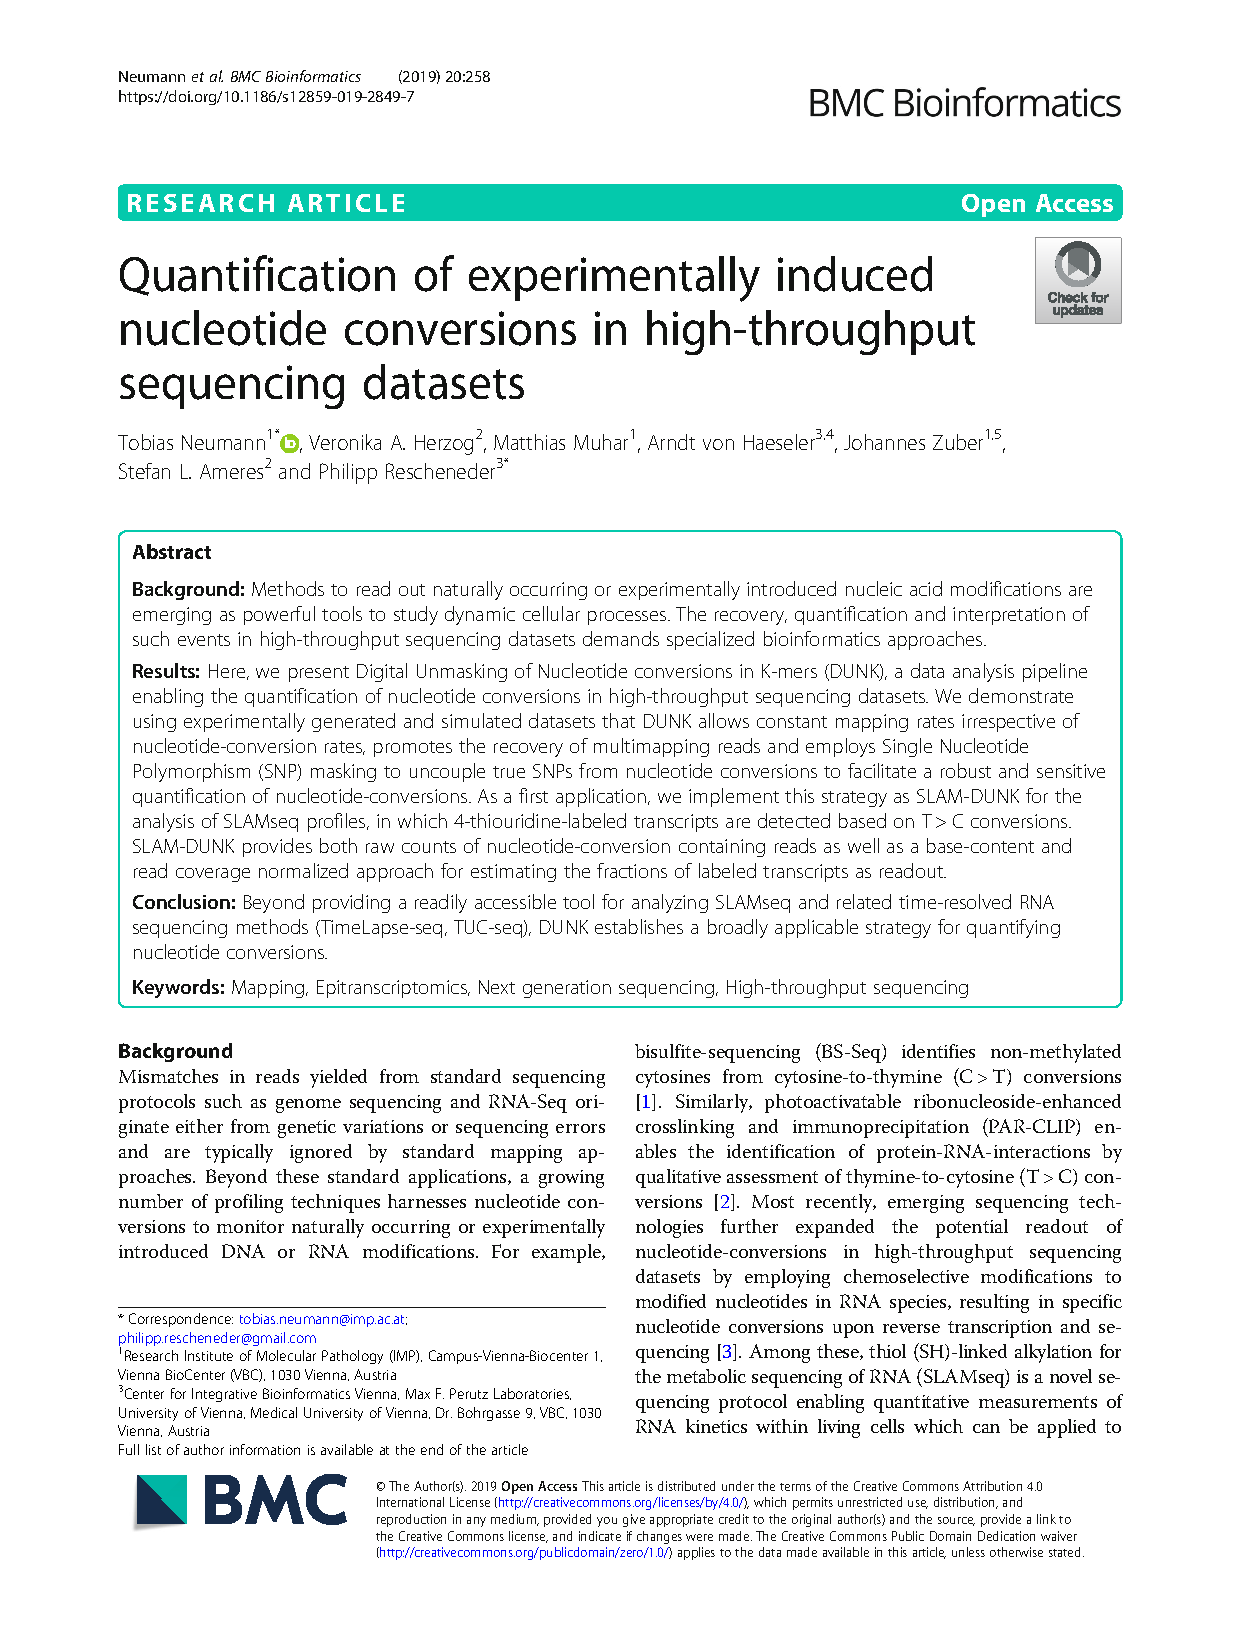
\includegraphics[page=1,scale=0.7]{papers/slamdunk_main.pdf}}

\includepdf[pages=2-,frame,scale=0.7,pagecommand={}]{papers/slamdunk_main.pdf}
